% ============================================================================
% CHƯƠNG 5: DOT PRODUCT VÀ MATRIX TRANSPOSE
% ============================================================================
\chapter{Dot Product và Matrix Transpose}
\label{chap:dot_transpose}

\section{Bài toán Dot Product (Tích vô hướng)}

\subsection{Định nghĩa}

Cho hai vector $\mathbf{A} = (a_0, a_1, ..., a_{n-1})$ và $\mathbf{B} = (b_0, b_1, ..., b_{n-1})$, tích vô hướng được định nghĩa:

\begin{equation}
\mathbf{A} \cdot \mathbf{B} = \sum_{i=0}^{n-1} a_i \times b_i = a_0 b_0 + a_1 b_1 + ... + a_{n-1} b_{n-1}
\end{equation}

\subsection{Ứng dụng}

Dot product được sử dụng rộng rãi trong:
\begin{itemize}
    \item \textbf{Machine Learning}: Tính toán trong neural networks
    \item \textbf{Computer Graphics}: Tính góc giữa hai vectors, chiếu sáng
    \item \textbf{Signal Processing}: Correlation, filtering
    \item \textbf{Physics}: Công, năng lượng
\end{itemize}

\subsection{Thuật toán Song song}

Dot product kết hợp hai patterns:
\begin{enumerate}
    \item \textbf{Element-wise multiplication}: Song song hoàn toàn (embarrassingly parallel)
    \item \textbf{Reduction (Sum)}: Cộng tất cả kết quả lại
\end{enumerate}

\begin{figure}[H]
\centering
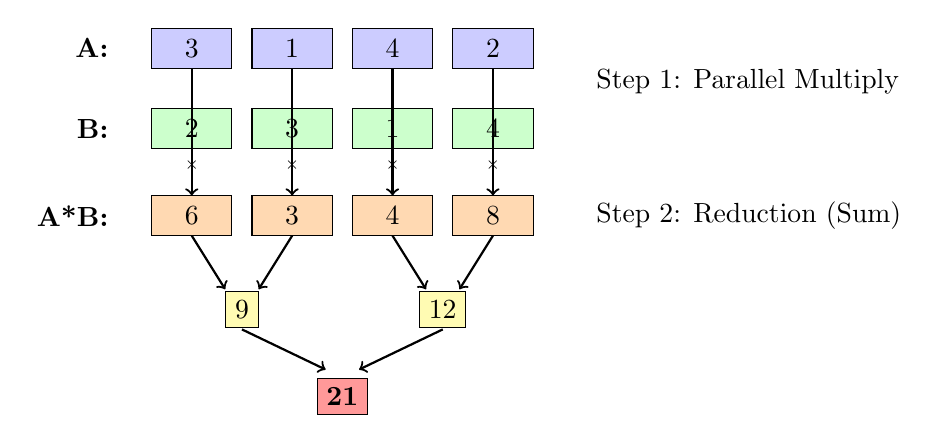
\begin{tikzpicture}[scale=0.85]
    % Vector A
    \node[left] at (-0.5, 3) {\textbf{A:}};
    \foreach \i/\v in {0/3, 1/1, 2/4, 3/2} {
        \draw[fill=blue!20] (\i*1.5, 2.7) rectangle ++(1.2, 0.6);
        \node at ({\i*1.5+0.6}, 3) {\v};
    }
    
    % Vector B
    \node[left] at (-0.5, 1.8) {\textbf{B:}};
    \foreach \i/\v in {0/2, 1/3, 2/1, 3/4} {
        \draw[fill=green!20] (\i*1.5, 1.5) rectangle ++(1.2, 0.6);
        \node at ({\i*1.5+0.6}, 1.8) {\v};
    }
    
    % Multiplication (parallel)
    \node[left] at (-0.5, 0.5) {\textbf{A*B:}};
    \foreach \i/\v in {0/6, 1/3, 2/4, 3/8} {
        \draw[fill=orange!30] (\i*1.5, 0.2) rectangle ++(1.2, 0.6);
        \node at ({\i*1.5+0.6}, 0.5) {\v};
    }
    
    % Arrows for multiplication
    \foreach \i in {0,1,2,3} {
        \draw[->, thick] ({\i*1.5+0.6}, 2.7) -- ({\i*1.5+0.6}, 0.8);
        \node[font=\tiny] at ({\i*1.5+0.6}, 1.25) {$\times$};
    }
    
    % Reduction tree
    \draw[->, thick] (0.6, 0.2) -- (1.1, -0.6);
    \draw[->, thick] (2.1, 0.2) -- (1.6, -0.6);
    \node[draw, fill=yellow!30] at (1.35, -0.9) {9};
    
    \draw[->, thick] (3.6, 0.2) -- (4.1, -0.6);
    \draw[->, thick] (5.1, 0.2) -- (4.6, -0.6);
    \node[draw, fill=yellow!30] at (4.35, -0.9) {12};
    
    % Final sum
    \draw[->, thick] (1.35, -1.2) -- (2.6, -1.8);
    \draw[->, thick] (4.35, -1.2) -- (3.1, -1.8);
    \node[draw, fill=red!40, font=\bfseries] at (2.85, -2.2) {21};
    
    % Labels
    \node[right] at (6.5, 2.5) {Step 1: Parallel Multiply};
    \node[right] at (6.5, 0.5) {Step 2: Reduction (Sum)};
    
\end{tikzpicture}
\caption{Thuật toán Dot Product: Multiply rồi Reduce}
\label{fig:dot_product_algo}
\end{figure}

\subsection{Cài đặt CUDA}

\begin{lstlisting}[caption={Dot Product Kernel với Reduction}, label={lst:dot_product_kernel}]
#define BLOCK_SIZE 256

__global__ void dotProductKernel(float *a, float *b, float *partialSums, int n) {
    __shared__ float sharedMem[BLOCK_SIZE];
    
    int tid = threadIdx.x;
    int idx = blockIdx.x * blockDim.x + threadIdx.x;
    
    // Buoc 1: Moi thread tinh a[idx] * b[idx]
    float temp = 0.0f;
    if (idx < n) {
        temp = a[idx] * b[idx];
    }
    sharedMem[tid] = temp;
    __syncthreads();
    
    // Buoc 2: Reduction trong shared memory
    for (int stride = blockDim.x / 2; stride > 0; stride >>= 1) {
        if (tid < stride) {
            sharedMem[tid] += sharedMem[tid + stride];
        }
        __syncthreads();
    }
    
    // Thread 0 ghi partial sum cua block
    if (tid == 0) {
        partialSums[blockIdx.x] = sharedMem[0];
    }
}

// Host code
float dotProduct(float *d_a, float *d_b, int n) {
    int gridSize = (n + BLOCK_SIZE - 1) / BLOCK_SIZE;
    float *d_partial, *h_partial;
    
    h_partial = (float *)malloc(gridSize * sizeof(float));
    cudaMalloc(&d_partial, gridSize * sizeof(float));
    
    dotProductKernel<<<gridSize, BLOCK_SIZE>>>(d_a, d_b, d_partial, n);
    cudaMemcpy(h_partial, d_partial, gridSize * sizeof(float), 
               cudaMemcpyDeviceToHost);
    
    // Cong partial sums tren CPU
    float result = 0.0f;
    for (int i = 0; i < gridSize; i++) {
        result += h_partial[i];
    }
    
    free(h_partial);
    cudaFree(d_partial);
    return result;
}
\end{lstlisting}

\section{Bài toán Matrix Transpose (Chuyển vị Ma trận)}

\subsection{Định nghĩa}

Cho ma trận $A$ kích thước $M \times N$, ma trận chuyển vị $A^T$ có kích thước $N \times M$ với:
\begin{equation}
A^T[j][i] = A[i][j], \quad \forall i \in [0, M-1], j \in [0, N-1]
\end{equation}

\begin{figure}[H]
\centering
\begin{tikzpicture}[scale=0.7]
    % Original matrix A
    \node[font=\bfseries] at (2, 4.5) {Ma trận A (3x4)};
    \foreach \i/\r in {0/{1,2,3,4}, 1/{5,6,7,8}, 2/{9,10,11,12}} {
        \foreach \j [count=\k from 0] in \r {
            \draw[fill=blue!20] (\k*1.2, {3-\i*1}) rectangle ++(1, 0.8);
            \node[font=\small] at ({\k*1.2+0.5}, {3.4-\i*1}) {\j};
        }
    }
    
    % Arrow
    \draw[->, very thick, red] (5.5, 1.5) -- (7, 1.5) node[midway, above] {$T$};
    
    % Transposed matrix
    \node[font=\bfseries] at (10, 4.5) {Ma trận $A^T$ (4x3)};
    \foreach \i/\r in {0/{1,5,9}, 1/{2,6,10}, 2/{3,7,11}, 3/{4,8,12}} {
        \foreach \j [count=\k from 0] in \r {
            \draw[fill=green!20] ({8+\k*1.2}, {3.5-\i*1}) rectangle ++(1, 0.8);
            \node[font=\small] at ({8.5+\k*1.2}, {3.9-\i*1}) {\j};
        }
    }
    
\end{tikzpicture}
\caption{Ví dụ chuyển vị ma trận}
\label{fig:transpose_example}
\end{figure}

\subsection{Vấn đề Memory Coalescing}

\textbf{Memory Coalescing} là kỹ thuật quan trọng để tối ưu truy cập bộ nhớ GPU. Khi các threads trong một warp truy cập các địa chỉ bộ nhớ liên tiếp, GPU có thể gộp nhiều truy cập thành một transaction.

\begin{figure}[H]
\centering
\begin{tikzpicture}[scale=0.65]
    % Memory layout
    \node[font=\bfseries] at (5, 5) {Row-major Memory Layout};
    \foreach \i in {0,...,11} {
        \draw[fill=gray!20] (\i*1, 4) rectangle ++(0.9, 0.8);
        \node[font=\tiny] at ({\i*1+0.45}, 4.4) {\i};
    }
    
    % Matrix view
    \node[font=\footnotesize] at (-2, 2) {Ma trận};
    \foreach \i in {0,...,2} {
        \foreach \j in {0,...,3} {
            \pgfmathtruncatemacro{\idx}{\i*4+\j}
            \draw[fill=blue!20] (\j*1, {2-\i*0.8}) rectangle ++(0.9, 0.7);
            \node[font=\tiny] at ({\j*1+0.45}, {2.35-\i*0.8}) {\idx};
        }
    }
    
    % Coalesced read (row access)
    \node[font=\footnotesize\bfseries, green!50!black] at (8, 2.5) {Coalesced Read (theo hàng)};
    \draw[very thick, green!50!black, ->] (5.5, 4) -- (5.5, 2.7);
    \draw[very thick, green!50!black] (0, 4) -- (3.9, 4);
    \node[font=\tiny, green!50!black] at (2, 3.6) {T0-T3 đọc liên tiếp};
    
    % Non-coalesced write (column access)
    \node[font=\footnotesize\bfseries, red] at (8, 0.5) {Non-coalesced Write (theo cột)};
    \foreach \i in {0,4,8} {
        \draw[thick, red, ->] ({\i*1+0.45}, 4) .. controls ({\i*1+0.45}, 3.5) .. ({8+\i/4*0.9+0.45}, 0.8);
    }
    \node[font=\tiny, red] at (10, 0) {T0-T3 ghi cách xa nhau};
    
\end{tikzpicture}
\caption{Vấn đề Memory Coalescing trong Transpose}
\label{fig:coalescing_issue}
\end{figure}

\subsection{Cài đặt cơ bản (Naive)}

\begin{lstlisting}[caption={Matrix Transpose - Naive Implementation}, label={lst:transpose_naive}]
__global__ void transposeNaive(float *in, float *out, int rows, int cols) {
    int ix = blockIdx.x * blockDim.x + threadIdx.x;
    int iy = blockIdx.y * blockDim.y + threadIdx.y;
    
    if (ix < cols && iy < rows) {
        // Read: coalesced (theo hang)
        // Write: non-coalesced (theo cot)
        out[ix * rows + iy] = in[iy * cols + ix];
    }
}
\end{lstlisting}

\subsection{Tối ưu với Shared Memory}

Sử dụng Shared Memory làm bước đệm để cả đọc và ghi đều coalesced:

\begin{lstlisting}[caption={Matrix Transpose với Shared Memory}, label={lst:transpose_shared}]
#define TILE_DIM 32

__global__ void transposeShared(float *in, float *out, int rows, int cols) {
    __shared__ float tile[TILE_DIM][TILE_DIM + 1]; // +1 de tranh bank conflicts
    
    int x = blockIdx.x * TILE_DIM + threadIdx.x;
    int y = blockIdx.y * TILE_DIM + threadIdx.y;
    
    // Read coalesced vao shared memory
    if (x < cols && y < rows) {
        tile[threadIdx.y][threadIdx.x] = in[y * cols + x];
    }
    __syncthreads();
    
    // Tinh toa do output (hoan vi block position)
    x = blockIdx.y * TILE_DIM + threadIdx.x;
    y = blockIdx.x * TILE_DIM + threadIdx.y;
    
    // Write coalesced tu shared memory
    if (x < rows && y < cols) {
        out[y * rows + x] = tile[threadIdx.x][threadIdx.y];
    }
}
\end{lstlisting}

\begin{figure}[H]
\centering
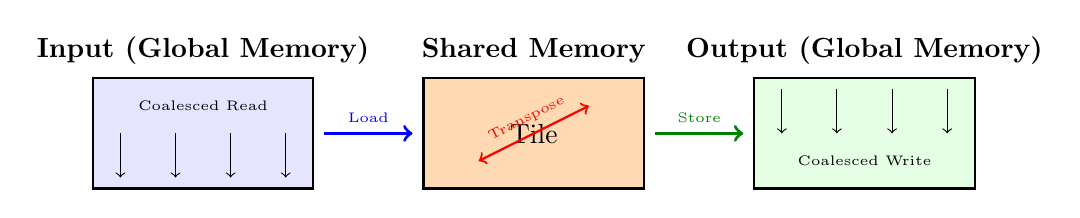
\begin{tikzpicture}[scale=0.7]
    % Input tile
    \node[font=\bfseries] at (2, 4.5) {Input (Global Memory)};
    \draw[fill=blue!10, thick] (0, 2) rectangle (4, 4);
    \draw[->] (0.5, 3) -- (0.5, 2.2);
    \draw[->] (1.5, 3) -- (1.5, 2.2);
    \draw[->] (2.5, 3) -- (2.5, 2.2);
    \draw[->] (3.5, 3) -- (3.5, 2.2);
    \node[font=\tiny] at (2, 3.5) {Coalesced Read};
    
    % Shared memory
    \node[font=\bfseries] at (8, 4.5) {Shared Memory};
    \draw[fill=orange!30, thick] (6, 2) rectangle (10, 4);
    \node at (8, 3) {Tile};
    
    % Output tile  
    \node[font=\bfseries] at (14, 4.5) {Output (Global Memory)};
    \draw[fill=green!10, thick] (12, 2) rectangle (16, 4);
    \draw[->] (12.5, 3.8) -- (12.5, 3);
    \draw[->] (13.5, 3.8) -- (13.5, 3);
    \draw[->] (14.5, 3.8) -- (14.5, 3);
    \draw[->] (15.5, 3.8) -- (15.5, 3);
    \node[font=\tiny] at (14, 2.5) {Coalesced Write};
    
    % Arrows
    \draw[->, very thick, blue] (4.2, 3) -- (5.8, 3) node[midway, above, font=\tiny] {Load};
    \draw[->, very thick, green!50!black] (10.2, 3) -- (11.8, 3) node[midway, above, font=\tiny] {Store};
    
    % Transpose in shared
    \draw[<->, thick, red] (7, 2.5) -- (9, 3.5) node[midway, above, font=\tiny, sloped] {Transpose};
    
\end{tikzpicture}
\caption{Tối ưu Transpose với Shared Memory}
\label{fig:transpose_shared}
\end{figure}

\section{So sánh hiệu năng}

\begin{table}[H]
\centering
\caption{So sánh các phương pháp Matrix Transpose}
\label{tab:transpose_comparison}
\begin{tabular}{@{}lccc@{}}
\toprule
\textbf{Ma trận} & \textbf{Naive (ms)} & \textbf{Shared Mem (ms)} & \textbf{Speedup} \\
\midrule
$1024 \times 1024$ & 0.245 & 0.112 & 2.19x \\
$2048 \times 2048$ & 0.892 & 0.378 & 2.36x \\
$4096 \times 4096$ & 3.456 & 1.423 & 2.43x \\
$8192 \times 8192$ & 13.78 & 5.623 & 2.45x \\
\bottomrule
\end{tabular}
\end{table}

\begin{figure}[H]
\centering
\begin{tikzpicture}
\begin{axis}[
    width=12cm,
    height=7cm,
    xlabel={Kích thước ma trận (N x N)},
    ylabel={Thời gian (ms)},
    legend pos=north west,
    grid=both,
    grid style={gray!30},
    ybar,
    bar width=15pt,
    symbolic x coords={1024, 2048, 4096, 8192},
    xtick=data,
    title={So sánh hiệu năng Matrix Transpose}
]
\addplot[fill=red!60] coordinates {
    (1024, 0.245)
    (2048, 0.892)
    (4096, 3.456)
    (8192, 13.78)
};
\addlegendentry{Naive}

\addplot[fill=green!60] coordinates {
    (1024, 0.112)
    (2048, 0.378)
    (4096, 1.423)
    (8192, 5.623)
};
\addlegendentry{Shared Memory}
\end{axis}
\end{tikzpicture}
\caption{Biểu đồ so sánh thời gian Transpose}
\label{fig:transpose_chart}
\end{figure}

\section{Cài đặt C\# (Bài tập midterm)}

\subsection{Dot Product với C\# Parallel}

\begin{lstlisting}[style=csharpstyle, caption={Dot Product với C\# Task/Channel}, label={lst:dotproduct_csharp}]
// Sequential
static double DotProductSequential(double[] A, double[] B) {
    double sum = 0.0;
    for (int i = 0; i < A.Length; i++)
        sum += A[i] * B[i];
    return sum;
}

// Thread/Task (Partitioning)
static double DotProductTask(double[] A, double[] B) {
    int numChunks = Environment.ProcessorCount;
    int chunkSize = (A.Length + numChunks - 1) / numChunks;
    double[] partialSums = new double[numChunks];
    Task[] tasks = new Task[numChunks];

    for (int c = 0; c < numChunks; c++) {
        int chunkIdx = c;
        int start = chunkIdx * chunkSize;
        int end = Math.Min(start + chunkSize, A.Length);

        tasks[c] = Task.Run(() => {
            double localSum = 0.0;
            for (int i = start; i < end; i++)
                localSum += A[i] * B[i];
            partialSums[chunkIdx] = localSum;
        });
    }
    Task.WaitAll(tasks);

    return partialSums.Sum();
}

// Channel (Producer-Consumer)
static async Task<double> DotProductChannel(double[] A, double[] B) {
    int numChunks = Environment.ProcessorCount;
    int chunkSize = (A.Length + numChunks - 1) / numChunks;
    var channel = Channel.CreateUnbounded<double>();

    // Producers
    var producers = new Task[numChunks];
    for (int c = 0; c < numChunks; c++) {
        int start = c * chunkSize;
        int end = Math.Min(start + chunkSize, A.Length);

        producers[c] = Task.Run(async () => {
            double localSum = 0.0;
            for (int i = start; i < end; i++)
                localSum += A[i] * B[i];
            await channel.Writer.WriteAsync(localSum);
        });
    }

    _ = Task.Run(async () => {
        await Task.WhenAll(producers);
        channel.Writer.Complete();
    });

    // Consumer
    double total = 0.0;
    await foreach (var partialSum in channel.Reader.ReadAllAsync()) {
        total += partialSum;
    }
    return total;
}
\end{lstlisting}

\subsection{Kết quả Benchmark C\#}

\begin{table}[H]
\centering
\caption{So sánh các phương pháp C\# (N = 1,000,000)}
\label{tab:csharp_benchmark_dottranspose}
\begin{tabular}{@{}lccc@{}}
\toprule
\textbf{Bài toán} & \textbf{Sequential} & \textbf{Task/Thread} & \textbf{Channel} \\
\midrule
Dot Product & 2.34 ms & 0.78 ms (3.0x) & 0.92 ms (2.5x) \\
Matrix Transpose (1K x 2K) & 4.56 ms & 1.23 ms (3.7x) & 1.45 ms (3.1x) \\
\bottomrule
\end{tabular}
\end{table}

\section{Kết luận chương}

Chương này đã trình bày hai bài toán quan trọng:

\textbf{Dot Product:}
\begin{itemize}
    \item Kết hợp element-wise multiply với reduction
    \item Sử dụng shared memory để tích lũy partial sums trong block
    \item Ứng dụng rộng rãi trong ML, graphics, physics
\end{itemize}

\textbf{Matrix Transpose:}
\begin{itemize}
    \item Vấn đề memory coalescing khi truy cập theo cột
    \item Giải pháp: Dùng shared memory làm bước đệm
    \item Tối ưu với \code{TILE\_DIM + 1} để tránh bank conflicts
    \item Speedup ~2.4x so với naive implementation
\end{itemize}

\textbf{C\# Parallel:}
\begin{itemize}
    \item Task/Thread pattern cho partitioning
    \item Channel pattern cho producer-consumer
    \item Speedup ~3x trên CPU multi-core
\end{itemize}
